\documentclass[twocolumn,10pt]{article}

\usepackage[margin=0.8in,bottom=1.25in,columnsep=.4in]{geometry}
\usepackage{amsmath}
\usepackage{amssymb}
\usepackage{listings}
\usepackage{color}
\usepackage{graphicx}
\usepackage{caption}
\usepackage{subcaption}

\DeclareMathOperator*{\argmin}{arg\,min}
\DeclareMathOperator*{\argmax}{arg\,max}

\definecolor{dkgreen}{rgb}{0,0.6,0}
\definecolor{gray}{rgb}{0.5,0.5,0.5}
\definecolor{mauve}{rgb}{0.58,0,0.82}
\lstset{frame=tb,
  language=Bash,
  aboveskip=3mm,
  belowskip=3mm,
  showstringspaces=false,
  columns=flexible,
  basicstyle={\small\ttfamily},
  numbers=none,
  numberstyle=\tiny\color{gray},
  keywordstyle=\color{blue},
  commentstyle=\color{dkgreen},
  stringstyle=\color{mauve},
  breaklines=true,
  breakatwhitespace=true,
  tabsize=3
}

\title{
	General solution for alphanumeric text-based CAPTCHAs\\
  using Convolutional Neural Networks\\ $ $\\
  \large 50.038 Computational Data Science \\
}

\author{
  Joel Huang\\
  \texttt{1002530}
  \and
  Karthic Harish Ragupathy\\
  \texttt{1002265}
  \and
  Ivan Zhou Yue\\
  \texttt{1002238}
}

\begin{document}
\maketitle

\begin{abstract}
We align ourselves to the arguments of~\cite{cc,readingtext,stark2015captcha,zhaocaptcha}, highlighting the ease of breaking alphanumeric CAPTCHAs today. CAPTCHAs are meant to be reverse Turing tests, implemented in order to differentiate humans from bots. Today, a number of sites still naively use alphanumeric CAPTCHAs as a first line of defence against automated attacks, flagging themselves as vulnerable targets to potential attackers. Recent advances in convolutional neural networks (CNNs) have produced the new state-of-the-art in object detection~\cite{resnet,fl}. Combined with long-known image segmentation and processing algorithms, old-school alphanumeric CAPTCHAs are solvable to a extremely high degree. In this paper, we aim to show that it is time to phase out alphanumeric text-based captchas once and for all.
\end{abstract}

\section{Introduction}
The problem of CAPTCHA breaking is important because it is essentially a contradiction to the web-based Turing test (and by extension, the reverse Turing test). In the last decade, the use of text-based CAPTCHAs to block automated requests have largely declined, due to improvements in the ability of paid automatic solvers, and the increasing accuracy of machine vision algorithms via convolutional neural networks, which makes it easy for any programmer to prepare and deploy a decently accurate model. However, many production-level systems have previously adopted text-based CAPTCHAs as security strategies and have not updated their systems with a more secure model.  Some common types of text-based CAPTCHAs are displayed in Fig. \ref{fig:captchaexamples}.

\subsection{Problem Framing}
We frame the CAPTCHA-breaking task as a character-level object detection problem. A correct solution involves producing a subset of characters, chosen from a set of 62 alphanumeric (A-Z, a-z, 0-9) characters that exactly matches the characters that were used to generate the CAPTCHA. We constrain the solution further as follows: the predicted string must match the original string’s length and sequence; and all characters are mutually exclusive, meaning that the prediction must be case-sensitive, so the model must be able to handle hard-to-distinguish characters like ‘o’, ‘O’ and ‘0’.

\begin{center}
\begin{figure*}
  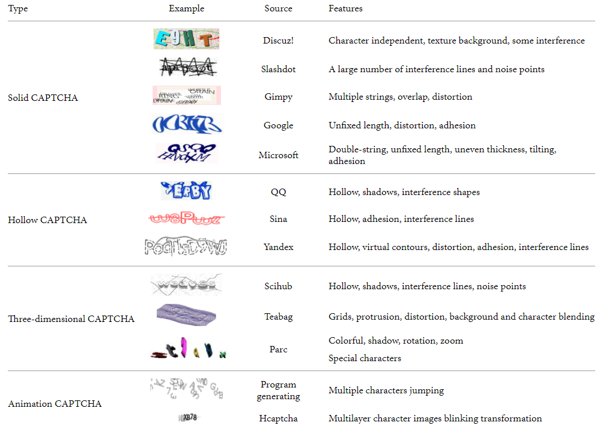
\includegraphics[width=\textwidth]{text_based_captcha.PNG}
  \caption{Common types of text-based CAPTCHAs used on the web}
  \label{fig:captchaexamples}
\end{figure*}
\end{center}

\subsection{Methodology}
Our training stage will involve a training set, which we describe in the next section. Input images pass through an Otsu preprocessor, which thresholds the images to remove noise, then are fed into the neural network for training. The test stage is similar, where the test set will also be fed through the Otsu preprocessor, then into the neural network for inference. We use different metrics for character-level prediction (IOUs, class-level mAP) and for accurate CAPTCHA string sequencing ($mAP^{len(captcha)}$). We also introduce a novel step, which we term unseen testing. In this step, our pipeline is fed CAPTCHA images that are totally unseen, independent of the training and test sets. The same metrics apply to evaluate our model.

\section{Dataset and Visualization}
\subsection{Terminology}
All text-based CAPTCHAs are technically ‘synthetic’, having been rendered at some point using different libraries and languages. However, in principle, we have no knowledge of the exact methods particular sites use to generate their CAPTCHAs. We thus consider scraped or downloaded CAPTCHAs as in-the-wild, or organic data, having been generated and deployed for actual use on production-level systems. We contrast this organic data to images that we are able to generate ourselves, which we will term as synthetic data.

\subsection{Gathering Organic Data}
The organic dataset is made up of roughly 15k text-based CAPTCHA images retrieved from the web. The organic portion of our dataset is merged from two online sources. We collected 15k real-world labelled CAPTCHAs of 2 different dimensions from these sources (see Fig. \ref{fig:organic}):
\begin{itemize}
\item 10k black and white, WordPress PHP plugin with over 1+ million downloads, of dimensions $(72 \times 24)$. These are scaled up to $(200 \times 75)$ for training.
\item 5k noiseless CAPTCHAs, scraped from online sources, of dimensions $(200 \times 75)$
\end{itemize}

\begin{center}
\begin{figure}
\centering
\begin{subfigure}{.4\columnwidth}
  \centering
  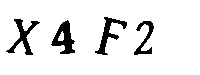
\includegraphics[width=.4\linewidth]{8908_X4F2.png}
  \caption{Black and white}
\end{subfigure}
\begin{subfigure}{.5\columnwidth}
  \centering
  
\includegraphics[width=.4\linewidth]{noiseless.png}
  \caption{Noiseless}
\end{subfigure}
\caption{Organic CAPTCHA classes}
\label{fig:organic}
\end{figure}
\end{center}

\subsection{Learning labels from Synthetic Data}
While our organic data is immensely valuable as real-world ground truths, we are unable to localize characters within the images in the current dataset. We hypothesize that synthetic data will be able to help us to solve this problem, inspired by synthetic data learning~\cite{synth}.
\\\\
For this task, we have written a custom Python CAPTCHA generation library that is able to generate character-based CAPTCHAs with variations in font, color, and spacing; carry out transformations like warping, vertical offset, rotation; and create irregularities in the form of background variation, point and line noise, and line and arc occlusion. Most importantly, we are able to create pixel-perfect localization labels for our synthetic data.

\begin{center}
\begin{figure}
\centering
\begin{subfigure}{.5\columnwidth}
  \centering
  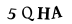
\includegraphics[width=.4\linewidth]{bw.PNG}
  \caption{Organic}
  \label{fig:sub1}
\end{subfigure}%
\begin{subfigure}{.5\columnwidth}
  \centering
  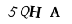
\includegraphics[width=.4\linewidth]{synthbw.png}
  \caption{Synthetic}
  \label{fig:sub2}
\end{subfigure}
\caption{Comparison between organic and synthetic}
\label{fig:test}
\end{figure}
\end{center}

\subsection{Deep learning for annotation}
In order to validate our hypothesis that we should be able to learn labels for our organic dataset, we analyzed the PHP portion of our dataset. The dataset draws characters exclusively from a set of variants of Gentium (regular, italic, bold and bold italic) with replacement, including random rotations and spacing within certain thresholds. We then generate 50k synthetic samples, which we argue are highly similar to the 10k organic samples, and learn localization labels on the organic set from the ones in the synthetic set, using the same architecture as our final model, RetinaNet~\cite{fl}. We then manually fixed any labels that were wrong, and fixed bounding boxes that were off. This task was made largely trivial because our proxy annotation model did an extremely good job, and enabled us a semi-automated method of gaining bounding box information for our entire organic dataset.

\subsection{Synthetic Data}
Early on, we noted that in this problem, in-the-wild, real-world CAPTCHAs have extremely small dissimilarity to synthetic data: the procedure to generate synthetic data is almost identical to the procedures used to generate ‘production-grade’ alphanumeric CAPTCHAs. Typically, a 4-6 character alphanumeric string is generated at pseudo-random, then rendered together with variable font families, font weights and sizes, positional offsets, typographic artifacts such as negative kerning, affine transformations, and filtering. There have been many instances of successful learning with synthetic data~\cite{readingtext,synth}.

To create diversity sufficient to replace the lack of organic data available, we modified the image parameters as follows:

\subsubsection{Uniform random character sampling}
We randomly sample alphanumeric characters, using the full range of 62 upper and lower case ASCII and single digit numerals.

\subsubsection{Noise generation}
We design \textbf{curves}, arc and line occlusions that occur randomly, creating $0-3$ horizontal cuts that pass through at least $50\%$ of the letters. We also introduce \textbf{dots}, creating $20-35$ dots scattered throughout the image. By creating these artifacts, we hope to increase the invariance to noise in our classification step.

\subsubsection{Color randomization}
Colors are randomly allocated within the RGB spectrum. For visibility, we constrain background colors to values above $(238, 238, 238)$ and foreground colors below $(200, 200, 200)$.

\subsubsection{Font selection}
We render the most common types of fonts in this experiment. In general, there are a few broad classes of fonts, including sans-serif, serif, slab, and monospace. We choose the most common sans-serif and serif fonts from the Google Fonts open-source directory. We picked Droid Sans Mono and Roboto for sans-serifs; and Gentium and Merriweather for serifs. We also introduce different font weights within the font families.

\subsubsection{Alignment and size}
The alignment of the strings are varied. Each of the characters may or may not be in the same line. We define curves with randomized parameters that are used to offset character heights.

\subsection{Visualizations}
    
Our final combined dataset consists of $50,000$ CAPTCHA images, with three main divisions: color, noiseless, and black and white. The table below describes each class of CAPTCHA and its characteristics, and the distribution is shown in Fig. \ref{fig:distribution}.
\begin{center}
\begin{tabular}{|c|c|c|} 
\hline
Class & Character count & Character types\\
\hline
Color & $4-6$ & Full alphanumeric\\
Noiseless & $6$ & Lowercase and digits\\
BW & $4$ & Uppercase and digits\\
\hline
\end{tabular}
\end{center}

\begin{center}
\begin{figure*}
  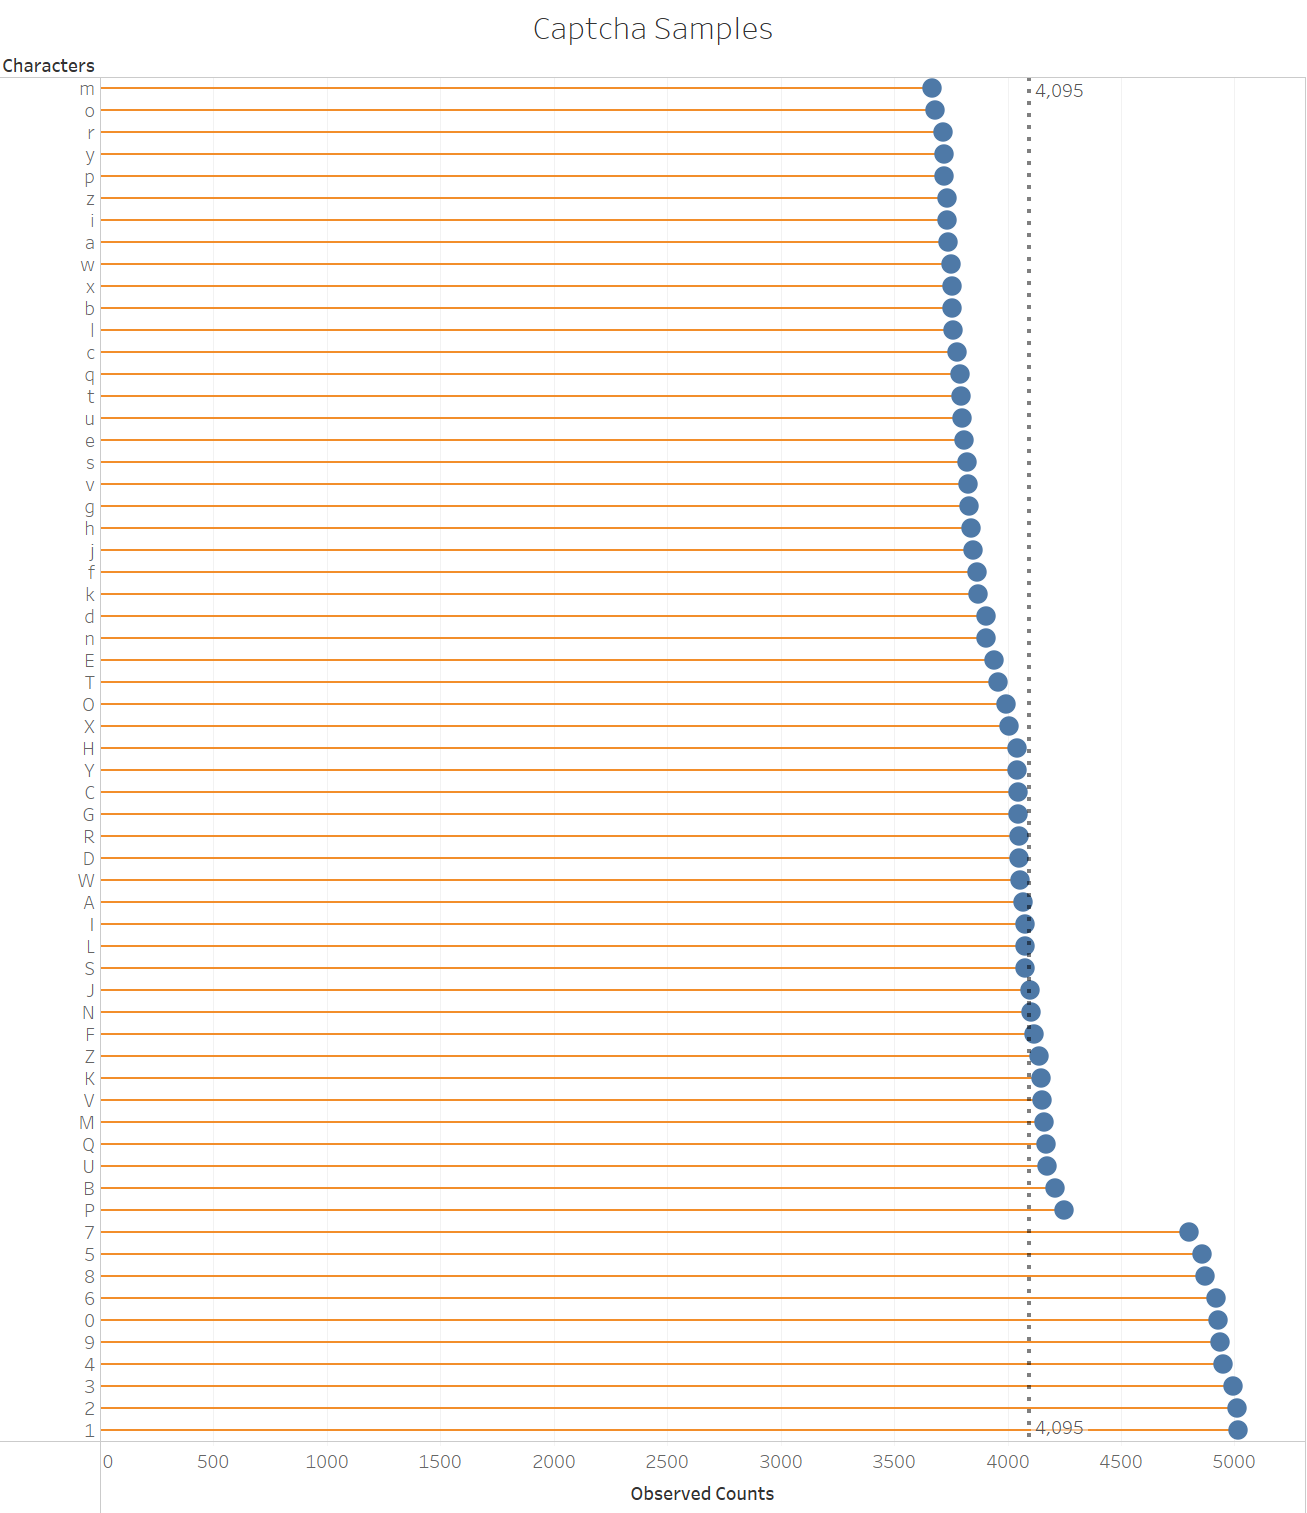
\includegraphics[width=\textwidth]{samples.png}
  \caption{Distribution of characters in dataset. Notice that the overall dataset is not uniform distributed. The observed counts for letters are significantly less than digits. This is because the lowercase letters are not rendered for the black and white class, uppercase letters are not rendered for the noiseless class, while digits are rendered for all classes. 
}
  \label{fig:distribution}
\end{figure*}
\end{center}

\subsubsection{Relationship analysis using PCA \& t-SNE}
In order to understand the relationship between the features in our dataset, we employ Principal Component Analysis (PCA) and t-distributed Stochastic Neighbour Embedding (t-SNE) to reduce the dimension of the images. Each character in the CAPTCHAs is segmented, extracted and resized to fit a ($60\times60$) pixels box (Fig. \ref{fig:pcachars}). Secondly, a threshold transformation is applied to convert the characters into black and white images with a singular RGB value, ranging from 0 to 255. This results in a 3600-dimensional vector of pixel values. PCA is used to reduce the dimensionality of each vector and to find directions (principal components) that contain the largest spread/subset of data points or information (variance) relative to all the other data points. t-SNE is used for the same purpose. A non-linear, probabilistic dimensionality reduction method whereby it aims to convert the Euclidean distances between points into conditional probabilities. A Student's-t distribution is then applied on these probabilities which serve as metrics to calculate the similarity between one datapoint to another. Our results can be seen in Fig. \ref{fig:pca} and Fig. \ref{fig:tsne}.

\begin{center}
\begin{figure}
  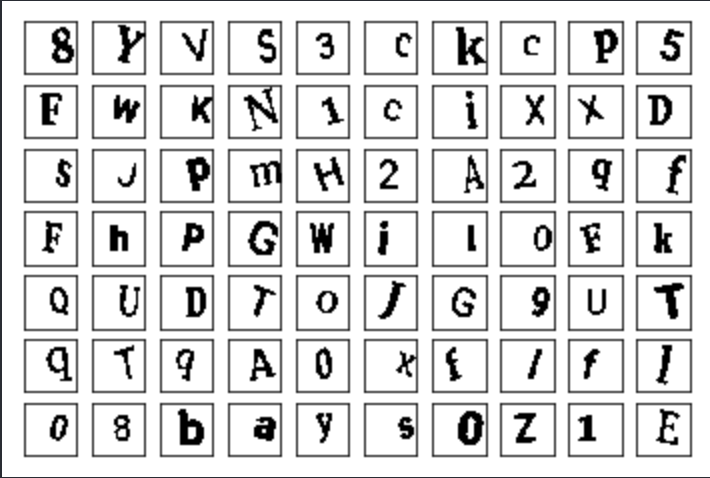
\includegraphics[width=\linewidth]{color_chars.png}
  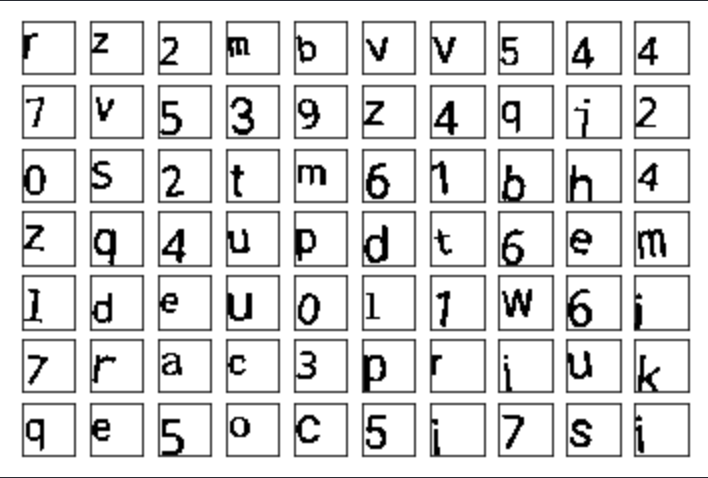
\includegraphics[width=\linewidth]{sutd_chars.png}
  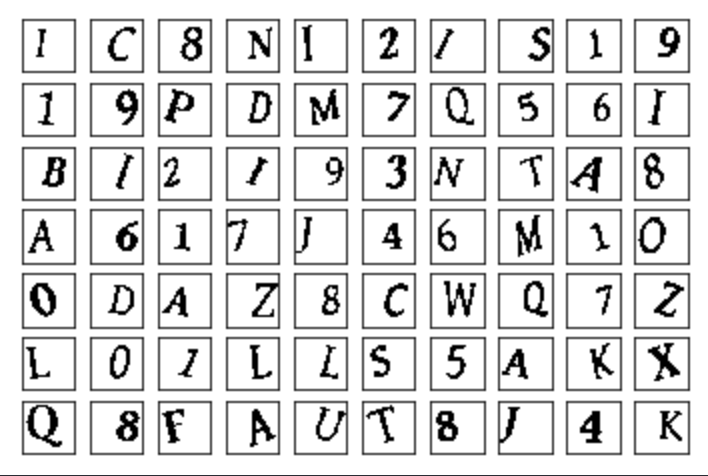
\includegraphics[width=\linewidth]{bw_chars.png}
  \caption{Color, noiseless and BW class characters for PCA and t-SNE}
  \label{fig:pcachars}
\end{figure}

\begin{figure}
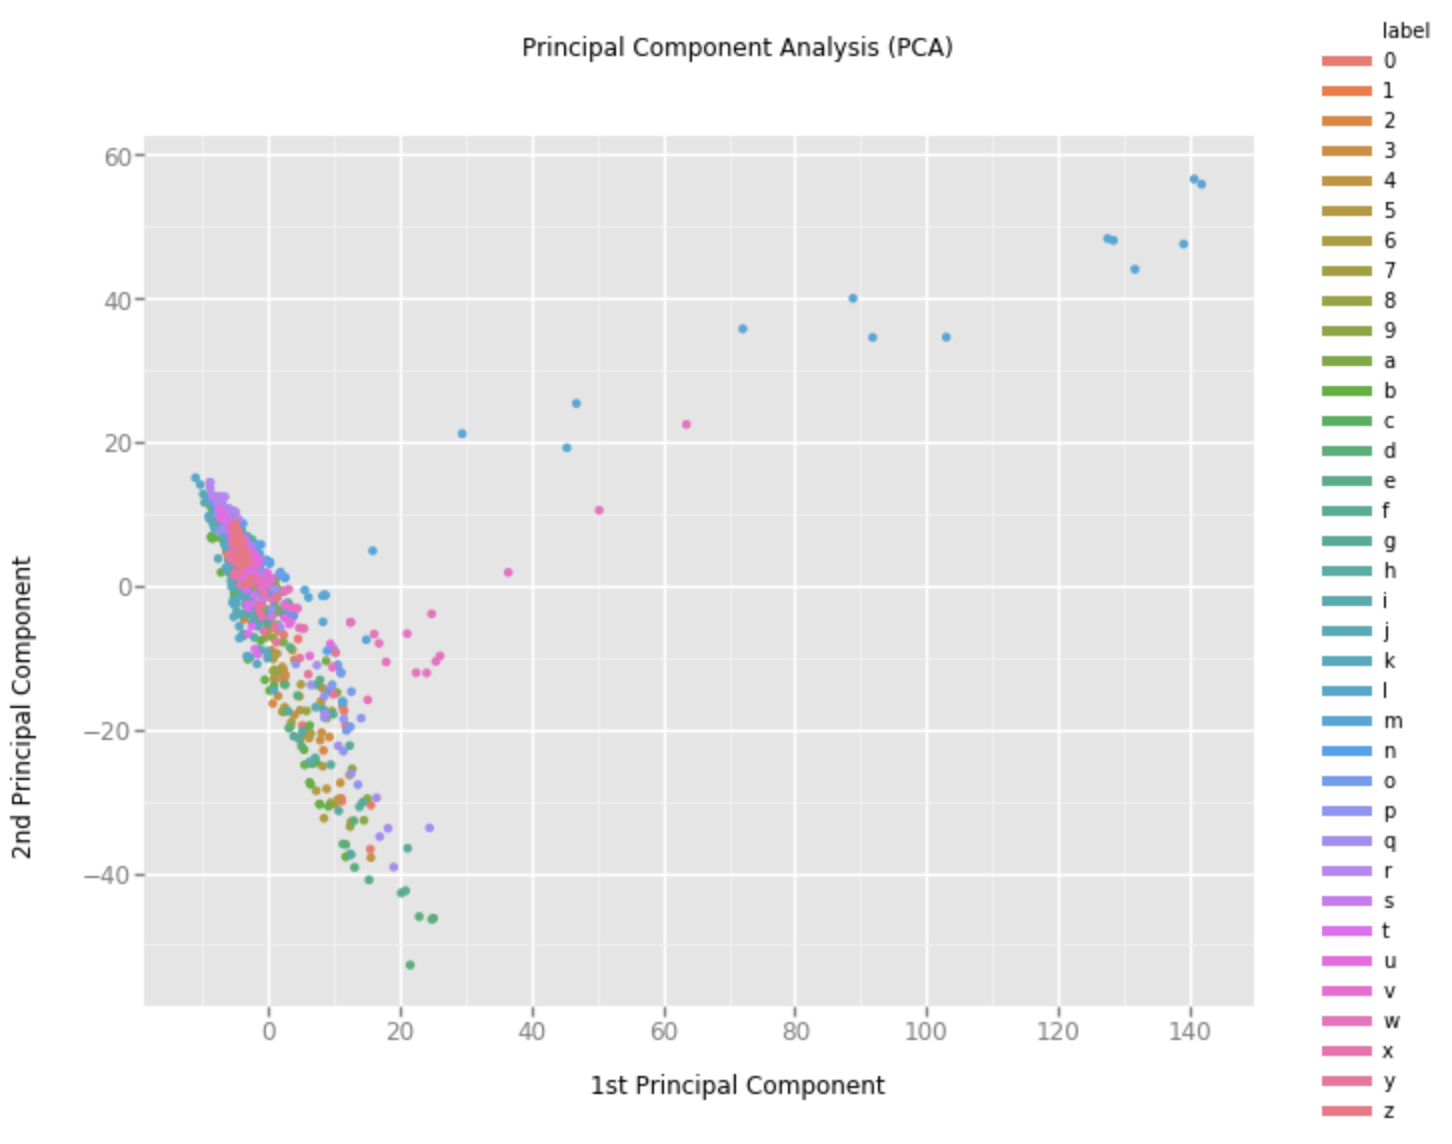
\includegraphics[width=\linewidth]{sutd_pca.png}
  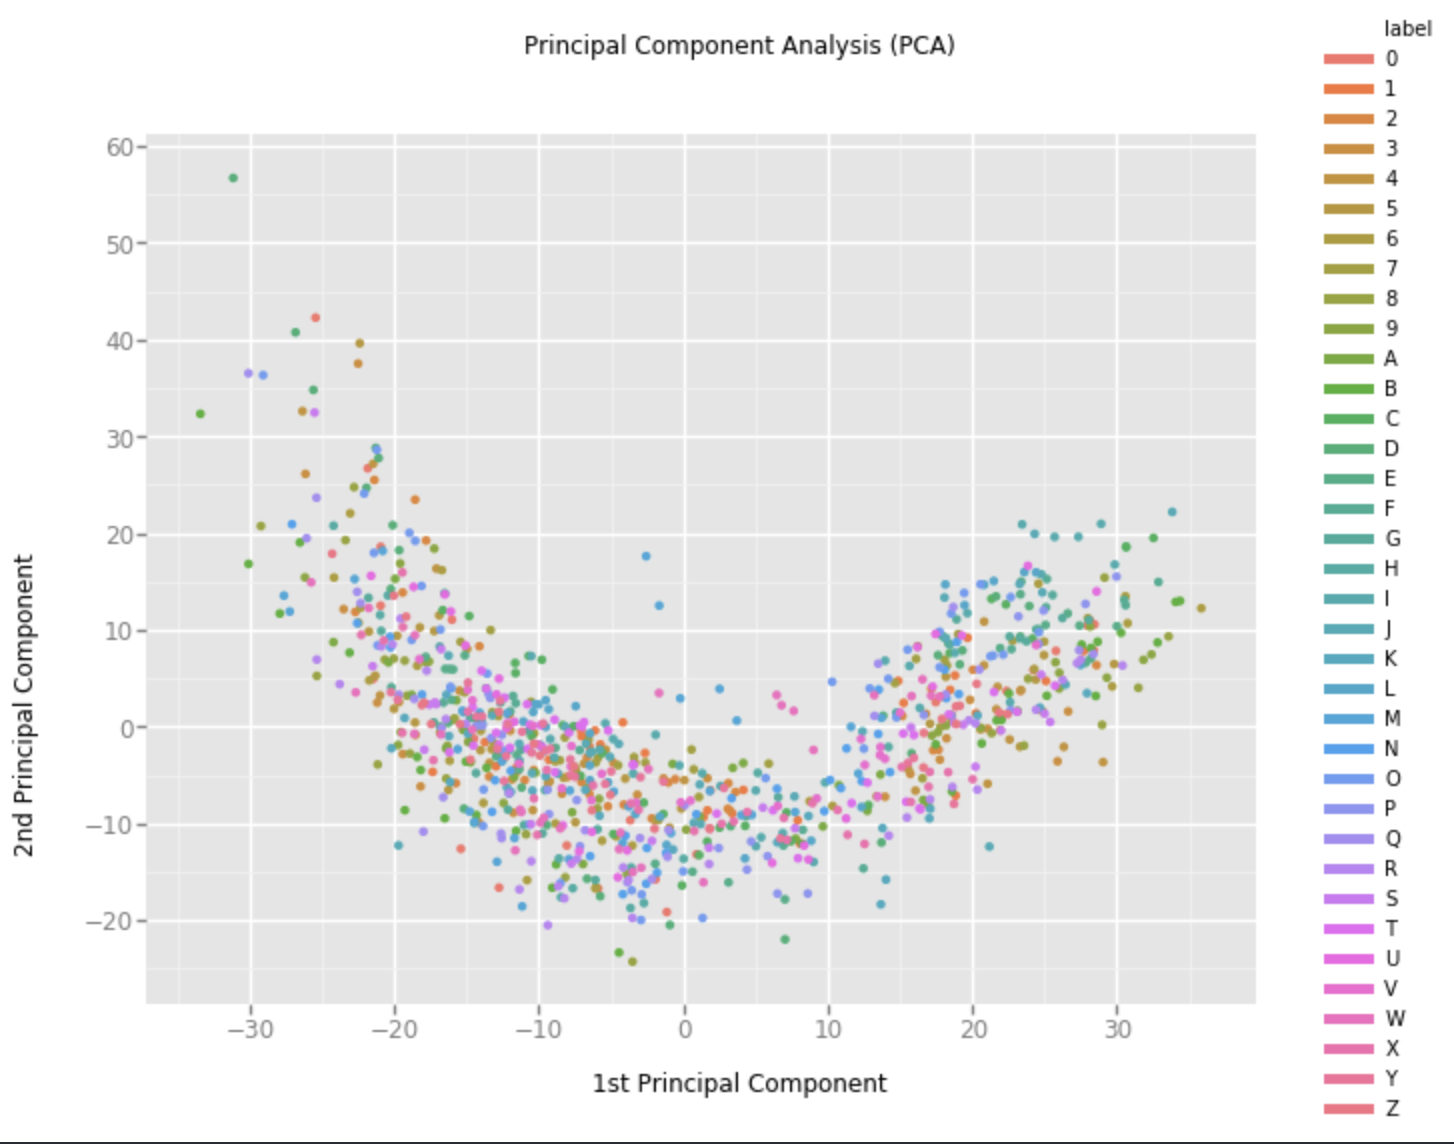
\includegraphics[width=\linewidth]{bw_pca.png}
  \caption{Principal components of the noiseless and BW sets}
  \label{fig:pca}
\end{figure}

\begin{figure}
  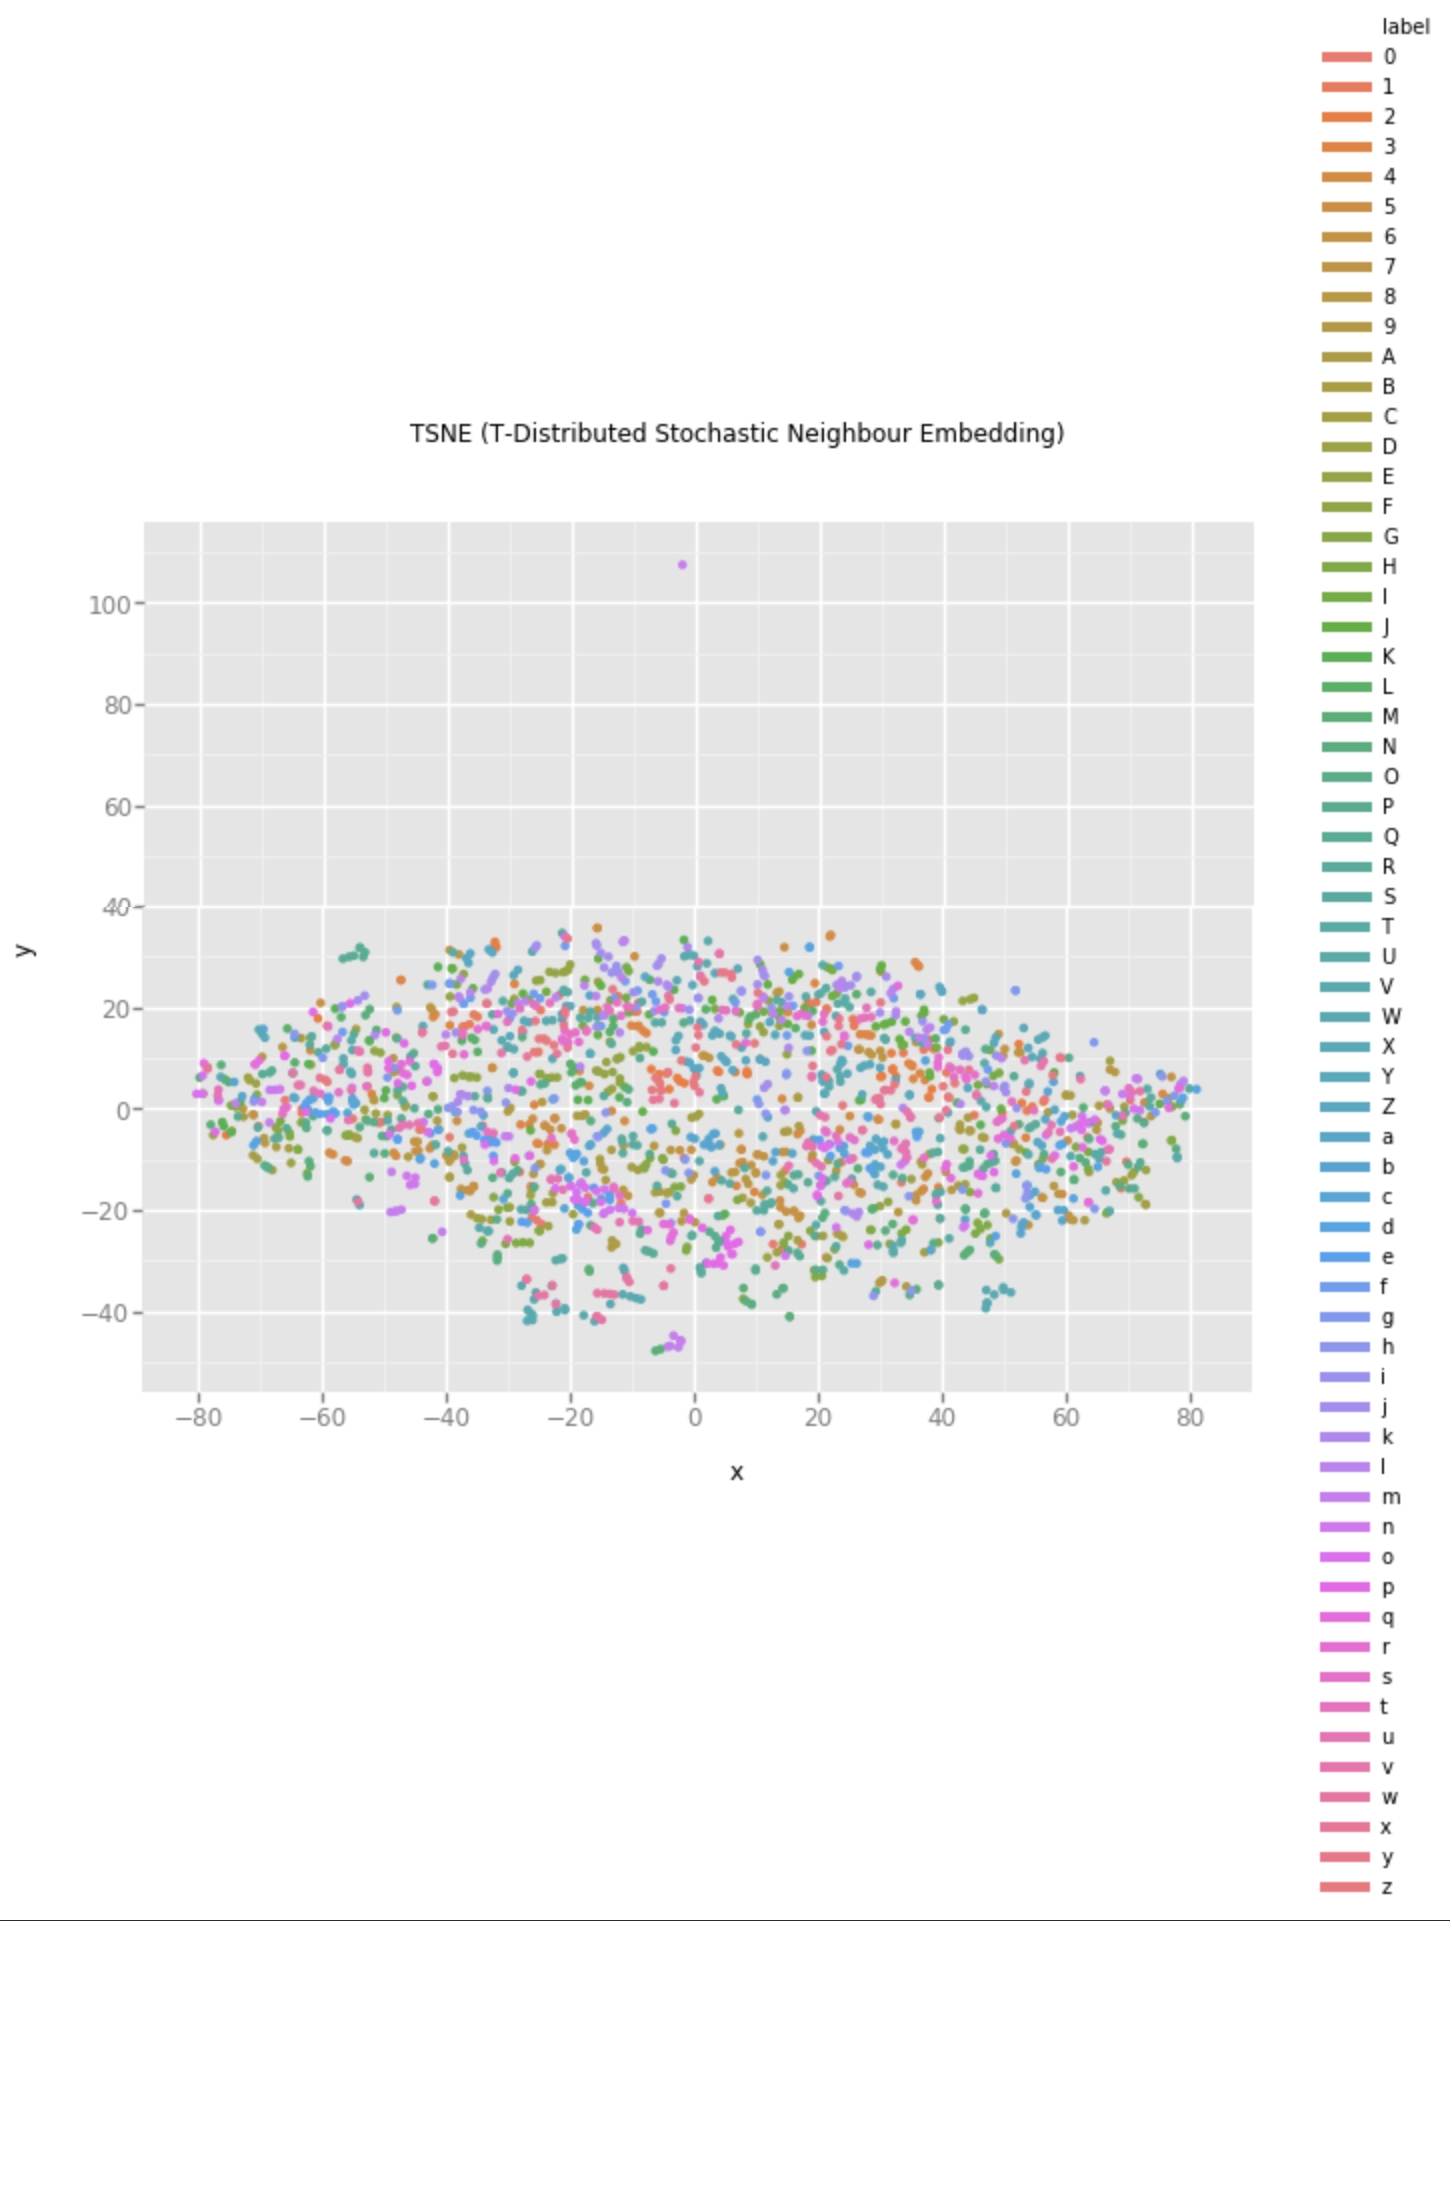
\includegraphics[width=\linewidth]{sutd_tsne.png}
  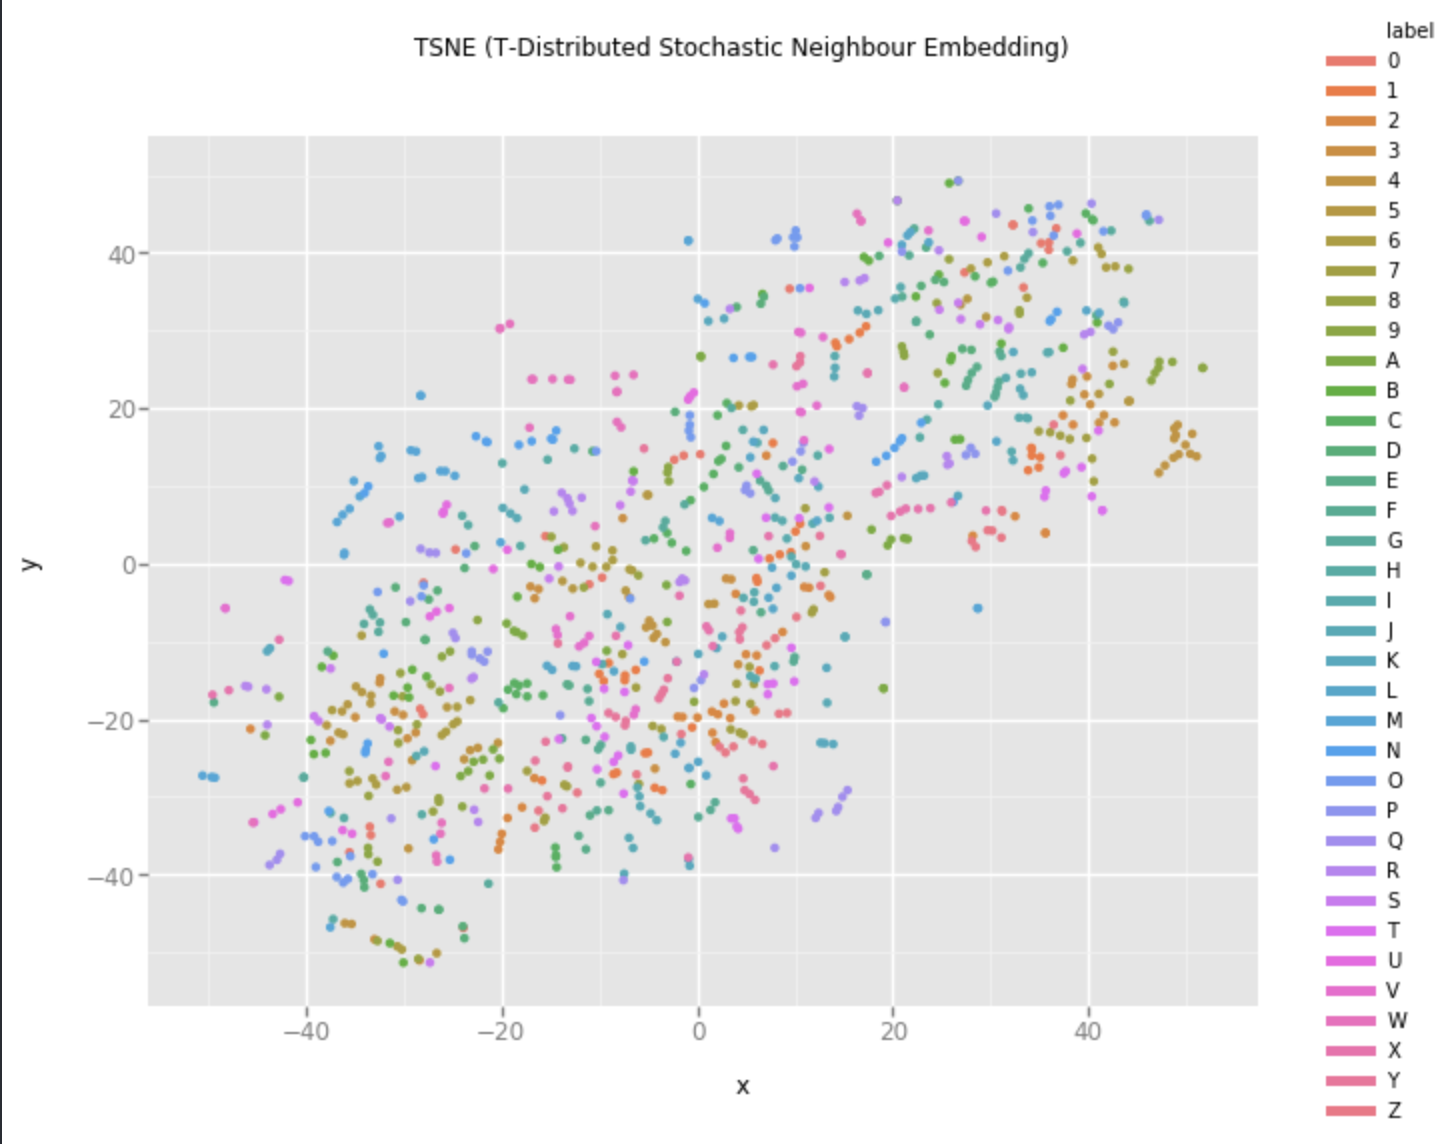
\includegraphics[width=\linewidth]{bw_tsne.png}
  \caption{t-SNE plots of the color and BW sets}
  \label{fig:tsne}
\end{figure}
\end{center}

As observed from the PCA scatter plots, there exist a few discernible clusters evinced from the collective blotches of colors. However, there is no clear distinction between the clusters. The t-SNE plots are more useful in distinguishing the various characters. For example, the left section of the plot represents characters with mostly straight line segments (l, T, i) while the top section represents characters with looops (o, O, 8, b).
Due to the close clustering and similarity between many of the characters, we conclude that the CAPTCHA images we’re dealing with are challenging and hence, we expect reduced accuracy scores for certain characters that are identical to others, such as o \& O, l \& I.

\section{Data Processing}
\subsection{Early attempts at algorithmic character segmentation}
We consider several preprocessing techniques, primarily to reduce noise. The objective is to simplify the input to a state were the segmentation algorithms can extract the letters. Some preprocessing algorithms we attempted include:
\begin{itemize} 
\item \textbf{Background/colour removal}. This is most useful against CAPTCHAs that use colour as a defence mechanism. It results in a grayscale image with the foreground pixels retaining their intensity and background pixels being white. However, there are CAPTCHA variants with gradient and pattern backgrounds, making an algorithmic background classification difficult.
\item \textbf{Upsampling}. Each pixel of the image is divided into subpixels, thus allowing finer control over the area that is affected by the segmentation algorithm. While upsampling might be useful for complex images like detailed photographs, less complex images like ours do not require it.
\item \textbf{Thresholding}. Removes pixels of low intensity (they are treated as noise), resulting in a binarized image. This is useful since most segmentation algorithms require a binarised input image. We eventually use an augmented form of thresholding in the final preprocessing algorithm.
\item \textbf{Line removal}. Eliminate straight segments that are not part of characters. This is particularly hard as our dataset has arc and line occlusion.
\end{itemize}

Our objective is to segment text from the background and attempt to split it into single character blocks. The goal of segmentation is to identify the location of the characters and extract them from the rest of the image. Published attacks use techniques that are specific to a particular CAPTCHA scheme. We attempted flood-filling segmentation, where an object is taken as a connected component created from neighbouring black pixels. Flood-filling segmentation takes a binarized image and returns the collection of objects found. However, this nearest-neighbour method doesn’t account for noise and compression artifacts. We found that some in-the-wild CAPTCHA sets contain JPEG artifacts, making flood-fill a poor choice as a boundary detector.

\subsection{Otsu Thresholding}
We choose Otsu thresholding~\cite{otsu} as it provides a robust binarization result, only occasionally letting noise through the filter. Consider a bimodal image, an image whose histogram has two peaks. For that image, Otsu thresholding computes a threshold value in the between the value of those peaks. Otsu's algorithm tries to find a threshold value $t$ which minimizes the weighted within-class variance given by the relation:
 
\begin{equation}
  \sigma^2_w = q_1(t) \cdot \sigma_1^2(t) + q_2(t) \cdot \sigma_2^2(t)
\end{equation}

where $q_i(t)$ is the cumulative sum of probabilities, and $\sigma_i^2$ is the variance. We first apply a 3x3 Gaussian blur to denoise the input, subsequently running Otsu thresholding on the filtered image. This results in a slightly better segmentation, as seen in Fig. \ref{fig:otsu}.

\begin{center}
\begin{figure}
\centering
\begin{subfigure}{.5\columnwidth}
  \centering
  
\includegraphics[width=.4\linewidth]{0_aWlV8o_original.png}
  \caption{Original colored}
\end{subfigure}%
\begin{subfigure}{.5\columnwidth}
  \centering
  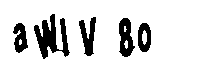
\includegraphics[width=.4\linewidth]{0_aWlV8o.png}
  \caption{After preprocessing}
\end{subfigure}
\caption{Pre- and post-Otsu thresholding}
\label{fig:otsu}
\end{figure}
\end{center}
 
All images are binarized according to the results of the segmentation phase mentioned above. A classifier is then used to recognise each of the characters. While early attacks against CAPTCHAs were using simple criteria such as the pixel count of the resulted objects, more recent attacks utilise machine learning classifiers that are trained on the output of the segmentation algorithm.

\section{Model Architecture}

We refer the state-of-the-art in object detection, using the RetinaNet~\cite{fl} meta-architecture for our classification and localization task. Typically, one-stage detectors like YOLO~\cite{yolov3} and SSD~\cite{ssd} demonstrate fast inference with low accuracy. We experiment casually with them, but find that RetinaNet is a faster, one-stage detector with comparable accuracy to slower two-stage detectors, like Feature Pyramid Networks (FPN)~\cite{fpn} and variants of Faster-RCNN~\cite{faster}. Here, we have two objectives, the classification of anchor boxes in the anchor set A, as one of 62 classes, and the regression from anchor boxes to ground-truth object boxes. We include the use of focal loss~\cite{fl} to reduce the contribution of easy classification examples during training and focus the model on hard examples:

\begin{equation}
  FL(p_t) = -(1-p_t)^\gamma \log (p_t)
\end{equation}

\begin{figure*}
  \centering
  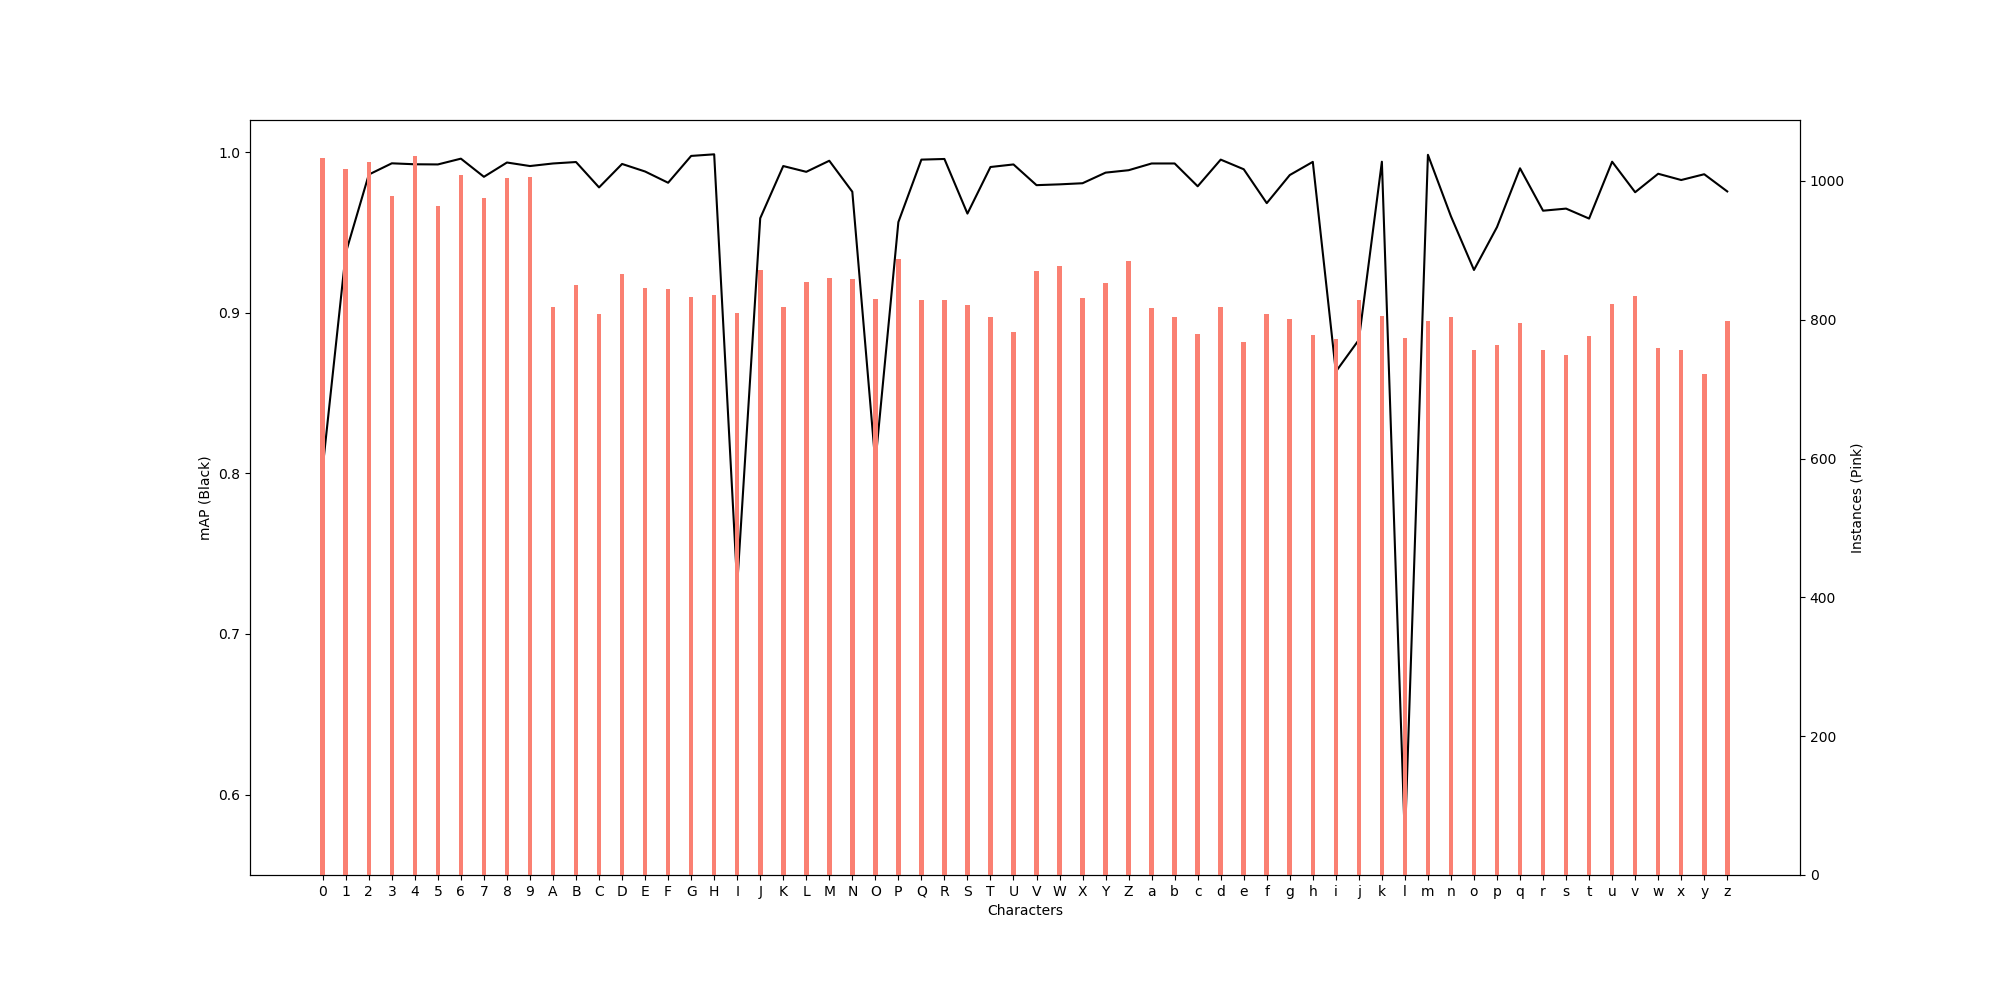
\includegraphics[width=\textwidth]{results.PNG}
  \caption{Results: mAP (black) and number test instances (pink) per character}
\label{fig:results}
\end{figure*}

\subsection{Backbone}
The one-stage RetinaNet uses a CNN-FPN backbone, and two heads for classification and regression. The backbone takes the job of computing the convolutional feature maps over the input image. We theorize that we can build a better model by going deep, since we are able to control the size of the dataset easily. We choose ResNet50~\cite{resnet} and augment it with a FPN, which creates a multi-scale feature pyramid instead of individual feature maps. This allows each layer to access different feature maps to detect objects at various scales.

\subsection{Classification}
The classification head predicts the probability of an alphanumeric character in the image, for each anchor $\in A$ and character class. The head is constructed with four 3x3 convolution layers with ReLU activations, followed by a final 3x3 convolution layer with $(classes \times A)$ filters, with a sigmoid activation for computing the probability score. The classification task on uses focal loss.

\subsection{Regression}
The regression head regresses the offset from each anchor box to the nearest ground truth object. The convolutional layers in the regression head are identical to the classification head, but the sub-network instead predicts the relative offset between the anchor and the true box. While the architecture is similar to the classification head, the parameters are kept separate. The regression task uses smooth L1 loss.

\subsection{Training}
We train with Keras, using the Adam~\cite{adam} optimizer for 32k iterations with a batch size of 40, and image augmentations including small amounts of rotation, translation, shear, and scaling. Flipping is not used for obvious reasons. 

\section{Evaluation Results}
We refer to the metrics discussed in Section 1.2. Our results are good on the testing set, reaching a mAP of 0.9624 after training for a total of 32k iterations. Based on Fig. \ref{fig:results}, we perform well on the test set on a per-character basis. However, in order to actually break the CAPTCHA, we have to successfully predict all the characters in the image. On average, for a 6-character CAPTCHA, this would mean that we only score $mAP^{len(captcha)} = 0.9624^6 = 0.7945$. Running the tests visually on test samples, as in Figs. \ref{fig:sample1}-\ref{fig:failure}, we find that our predictions are extremely accurate. We then run inference on the unseen set, with an example shown in Fig. \ref{fig:unseen}, to surprising results. Given these results, we are confident that with additional training on even more variants of text-based CAPTCHAs, this network will maintain its high mAP on test sets, while becoming even more robust to unseen data.

\begin{figure*}
  \centering
  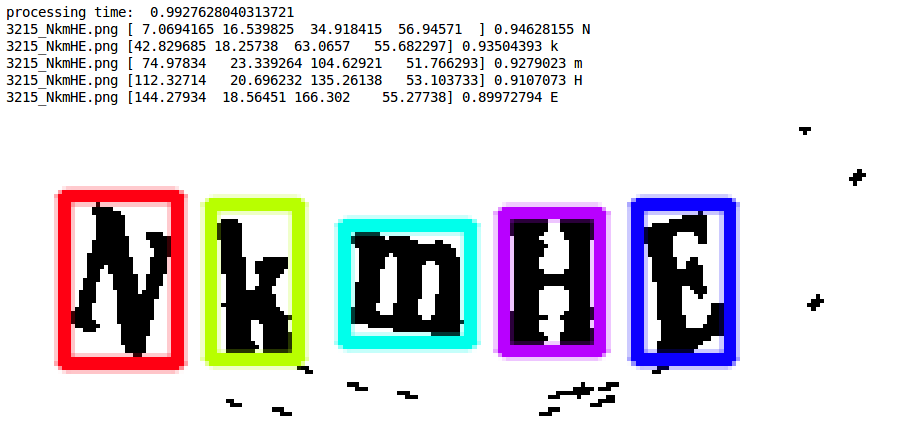
\includegraphics[width=\linewidth]{resultscolor.png}
  \caption{A sample test result on the color set}
  \label{fig:sample1}
\end{figure*}

\begin{figure*}
  \centering
  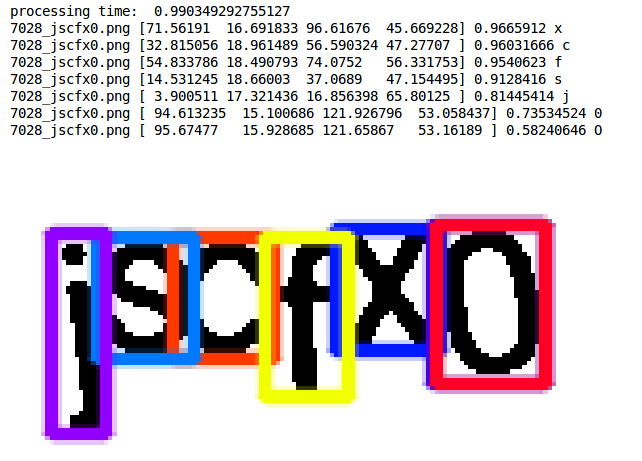
\includegraphics[width=.8\linewidth]{resultsnoiseless.png}
  \caption{A sample test result on the noiseless set}
  \label{fig:sample2}
\end{figure*}

\begin{figure*}
  \centering
  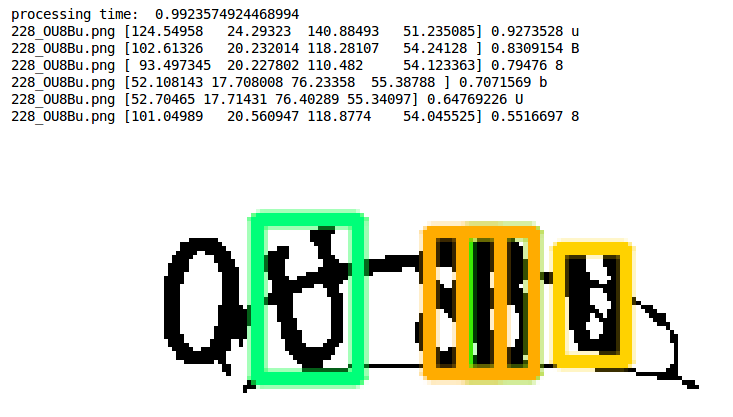
\includegraphics[width=\linewidth]{failurecolor.png}
\caption{Failure case on the color set, the only set with noise. We are unable to produce a failure case example for the noiseless and BW sets.}
\label{fig:failure}
\end{figure*}

\begin{figure*}
  \centering
  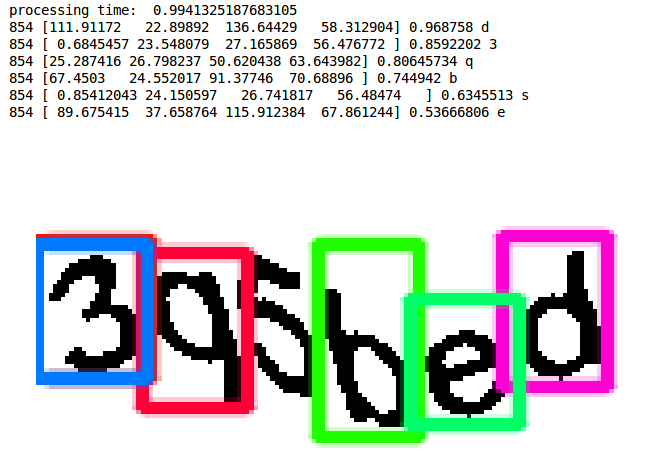
\includegraphics[width=\linewidth]{unseen.png}
\caption{A test on the unseen set. This CAPTCHA type has never been seen by our model during training. Of the 6 characters in this string, 3q5bed, we are able to correctly predict 5 characters: 3, q, b, e, and d.}
\label{fig:unseen}
\end{figure*}


\section{Conclusion}
Websites must stop using alphanumeric CAPTCHAs as a first line of defence against automated attacks. We show that a simple method to solve alphanumeric CAPTCHAs, even on unseen data, is available to anyone with basic knowledge of image processing and machine learning. It is time to phase out alphanumeric text-based captchas once and for all.

\bibliography{main}{}
\bibliographystyle{abbrv}
\end{document}